\chapter{Ciclo di Deming}\label{CicloDiDeming}
Noto anche come ciclo \textbf{\textit{PDCA}}, acronimo di Plan-Do-Check-Act.
Si tratta di un metodo di gestione iterativo suddiviso in quattro fasi che vengono utilizzato per il continuo controllo e miglioramento dei processi e prodotti.
Le fasi derivano dall’acronimo sopracitato:
\begin{itemize}
	\item \textbf{P - Plan}:  ovvero \textbf{\textit{Pianificazione}}. In questa fase vengono stabiliti gli obiettivi e i processi necessari per il raggiungimento dei risultati, coerenti con quanto atteso.
	Serve una pianificazione curata nei minimi dettagli, inoltre è preferibile predisporre miglioramenti su scala ridotta in modo da poter avere la situazione più sotto controllo.
	\item \textbf{D - Do}: tradotto \textbf{\textit{Fare}}. Avviene l’esecuzione del piano deciso nella fase precedente.
	Questo step è molto importante anche perché è necessario raccogliere i dati per l’analisi che sarà destinata alle due fasi successive.
	\item \textbf{C - Check}: Fase di \textbf{\textit{Controllo}}. I dati raccolti e misurati nella fase \textit{Do} ora vengono analizzati e controllati per verificare la congruenza con quelli aspettati, come negli obiettivi del \textit{Plan}.
	Inoltre in questa fase si cercano anche eventuali deviazioni del piano concordato per eventualmente cambiarlo per renderlo migliore.
	\item \textbf{A - Act}: \textbf{\textit{Agire}}. Ultima fase del ciclo. Ora ci si aziona per rendere definitivo o migliorare il processo. Vengono richieste azioni correttive nel caso in cui i dati raccolti abbiano significative differenze tra quelli attesi. 
	Al termine di questa fase il ciclo viene chiuso e tramite le decisioni prese verrà creata una nuova fase di \textit{Plan} che farà ripartire questo meccanismo.
\end{itemize}
\begin{figure}[!ht]
	\begin{center}
		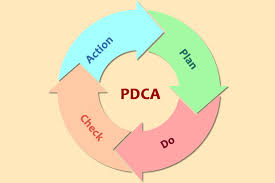
\includegraphics[width=0.48\linewidth]{../immagini/Ciclo_di_Deming.jpg}
		\caption{Rappresentazione del Ciclo di Deming}
	\end{center}
\end{figure}
